% Caso 02 — Problema de Sitnikov
\subsection{Caso 02: Problema de Sitnikov}
\begin{frame}{Resultados — Caso 02: Problema de Sitnikov}
    \textbf{Descripción:} problema clásico de caos determinista; dos estrellas orbitan en el plano XY mientras un tercer cuerpo oscila en el eje Z perpendicular.\\
    \vspace{0.2cm}
    {\small
    \textbf{Configuración del experimento:}
    \begin{itemize}
        \item Horizonte de simulación: $t_{short}=0.5$ años, $t_{long}=4.0$ años.
        \item Integrador: \texttt{IAS15} con paso $\Delta t=2\times10^{-4}$ años.
        \item Masas originales: $(0.8,\ 1.2,\ 2.5\times10^{-6})$ M$_\odot$.
        \item Optimización: población 180, 50 épocas, $\omega_{periodicidad}=0.05$.
        \item \textbf{Resultado:} Masas optimizadas $(0.819,\ 1.200,\ 2.5\times10^{-6})$ M$_\odot$.
        \item Reducción de caos: $\lambda_{inicial}=-0.98 \rightarrow \lambda_{opt}=-15.71$.
    \end{itemize}
    }
\end{frame}

\begin{frame}{Caso 02 — Evolución del exponente de Lyapunov}
    \vspace{0.1cm}
    \begin{center}
        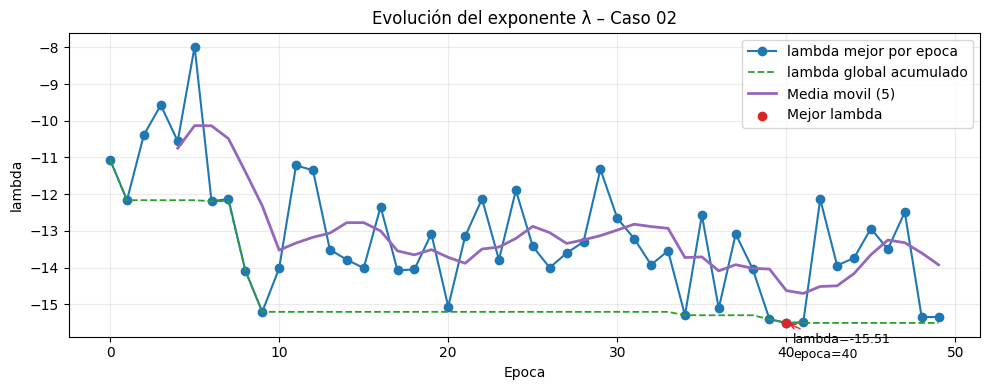
\includegraphics[width=0.85\textwidth, height=0.70\textheight, keepaspectratio]{img/resultados/caso02-evolucion_exponente.png}
    \end{center}
    \vspace{0.2cm}
    {\small Evolución del exponente de Lyapunov mostrando estabilización progresiva del sistema.~\textit{Autoría Propia}}
\end{frame}

\begin{frame}{Caso 02 — Video Comparación de trayectorias}
    \vspace{0.1cm}
    \begin{center}
        \href{run:img/resultados/vids/Caso02-Comparativa.mp4}{%
            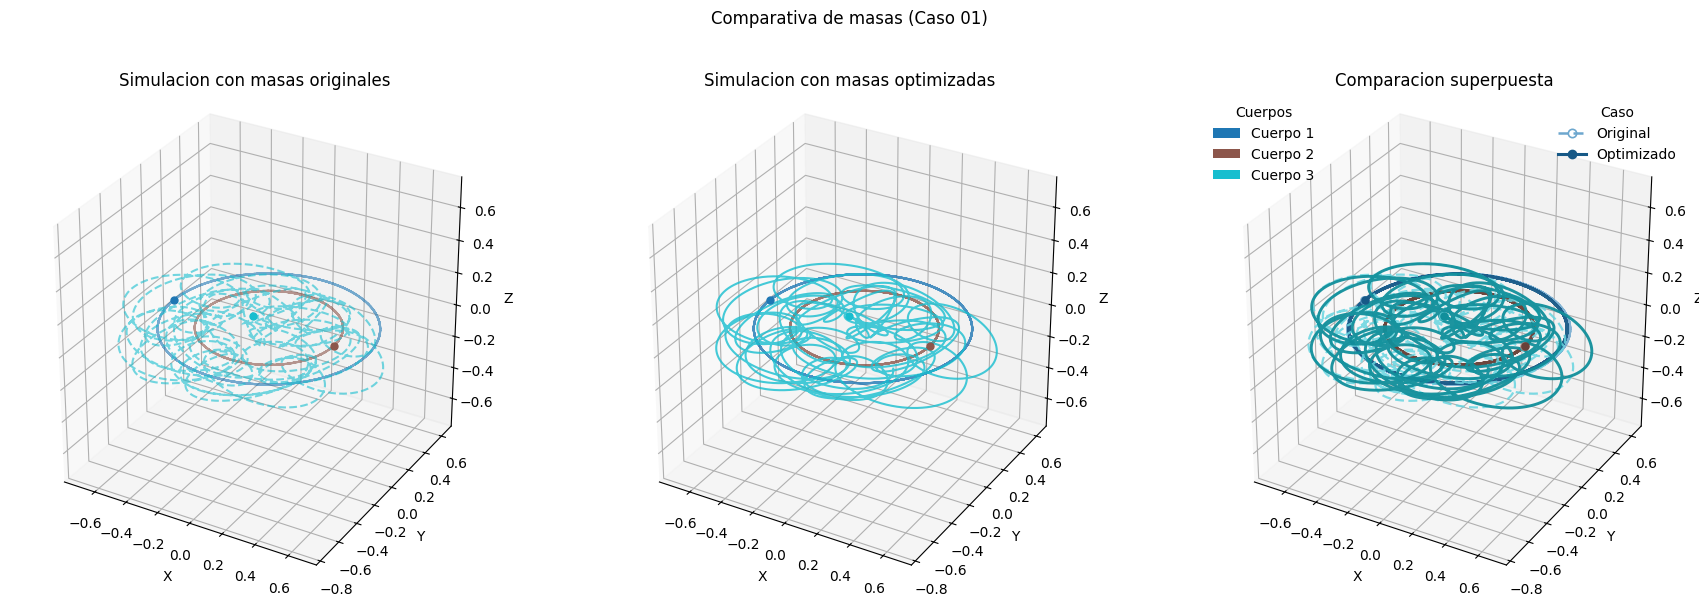
\includegraphics[width=0.85\textwidth, height=0.70\textheight, keepaspectratio]{img/resultados/caso02-comparativa_trayectoria.png}
        }
    \end{center}
    \vspace{0.2cm}
    {\small \textcolor{blue}{Clic en la imagen} para abrir el video comparativo en el reproductor del sistema.~\textit{Autoría Propia}}
\end{frame}